\begin{figure*}[t]
\centering
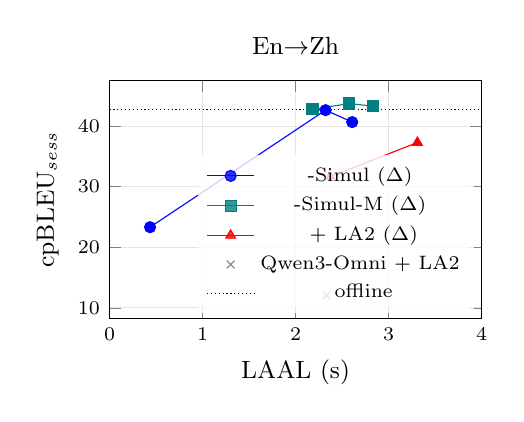
\begin{tikzpicture}\begin{axis}[width=0.52\textwidth, height=4.6cm, xlabel={LAAL (s)}, ylabel={cpBLEU$_\text{sess}$}, title={En$\rightarrow$Zh}, title style={font=\small}, tick label style={font=\scriptsize}, label style={font=\small}, xmin=0, xmax=4, enlarge y limits=0.12, grid=major, grid style={gray!20}, legend style={font=\scriptsize, at={(0.98,0.02)}, anchor=south east, draw=none, fill=white, fill opacity=0.8, text opacity=1}]
\addplot[blue, mark=*] coordinates {(0.435,23.31) (2.323,42.63) (2.609,40.66)}; \addlegendentry{\sys{}-Simul ($\Delta$)}
\addplot[teal, mark=square*] coordinates {(2.183,42.79) (2.579,43.72) (2.832,43.29)}; \addlegendentry{\sys{}-Simul-M ($\Delta$)}
\addplot[red, mark=triangle*] coordinates {(2.373,31.64) (3.310,37.29)}; \addlegendentry{\sys{} + LA2 ($\Delta$)}
\addplot[gray, only marks, mark=x] coordinates {(2.333,12.07)}; \addlegendentry{Qwen3-Omni + LA2}
\addplot[black, densely dotted, domain=0:4, samples=2] {42.81}; \addlegendentry{\sys{} offline}
\end{axis}\end{tikzpicture}
\hfill
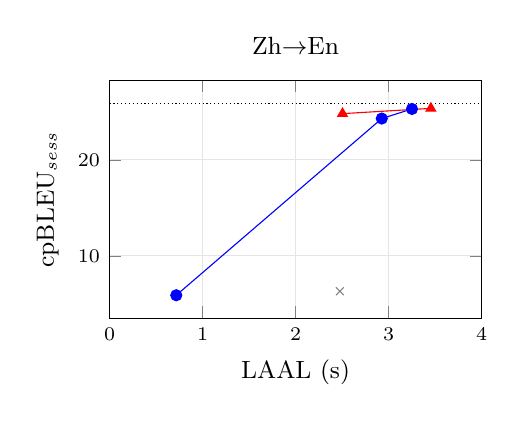
\begin{tikzpicture}\begin{axis}[width=0.52\textwidth, height=4.6cm, xlabel={LAAL (s)}, ylabel={cpBLEU$_\text{sess}$}, title={Zh$\rightarrow$En}, title style={font=\small}, tick label style={font=\scriptsize}, label style={font=\small}, xmin=0, xmax=4, enlarge y limits=0.12, grid=major, grid style={gray!20}]
\addplot[blue, mark=*] coordinates {(0.717,5.89) (2.927,24.30) (3.252,25.30)};
\addplot[red, mark=triangle*] coordinates {(2.505,24.81) (3.455,25.36)};
\addplot[gray, only marks, mark=x] coordinates {(2.476,6.31)};
\addplot[black, densely dotted, domain=0:4, samples=2] {25.86};
\end{axis}\end{tikzpicture}
\caption{Latency--quality trade-off (text) over the read interval $\Delta\in\{0.5,1,2\}$\,s (left to right).
\sys{}-Simul is trained at $\Delta=1$\,s, \sys{}-Simul-M at mixed intervals (En$\rightarrow$Zh). The dotted line is the offline \sys{}. Numbers in Table~\ref{tab:tradeoff}.}
\label{fig:tradeoff}
\end{figure*}
